\documentclass{beamer}
\usefonttheme{professionalfonts}
%\usetheme{Rochester}
%\usetheme{AnnArbor}
\usetheme{Szeged}
\useoutertheme{infolines}
\usecolortheme{dolphin}
\usepackage{graphicx}
% \usepackage[english]{babel}
\usepackage{hyperref}
\usepackage{multicol}
\usepackage{color}
\usepackage{xcolor}
%\usepackage{smartdiagram}


%\definecolor{carmine}{rgb}{0.59, 0.0, 0.09}
\usepackage{amsmath} 

\usepackage{graphicx}
\usepackage{tikz}
\usetikzlibrary{shapes.callouts}
\usepackage{multirow}

\usepackage[utf8]{inputenc}

\usepackage{enumerate}
\usepackage[shortlabels]{enumitem}
\usepackage{amsmath,amsthm,amssymb,amsfonts,mathrsfs,latexsym,stmaryrd}
\usepackage{tcolorbox}

\usepackage{color} 
\usepackage{amssymb, amsmath, amsbsy}
\usepackage{adjustbox,lipsum}
\usepackage{placeins}

\usepackage{textpos}
\usepackage{wrapfig}
\usepackage[spanish, es-tabla]{babel}

\usepackage{caption}
\setlength{\parindent}{0pt}
% Beamer already loads hyperref; avoid reloading it with conflicting options.

\usepackage{url}
\usepackage{float}
\usepackage{tikz}
\usetikzlibrary{patterns}


\title[ICS-294]{Econometría ICS-294\\ \small{Clase 2: Modelo de Regresi\'on Lineal Simple}}

\author{Francisco Alfaro Medina}
\institute[USM]
{Universidad Técnica Federico Santa María\\ % Your institution for the title page
	\medskip
	\textit{} % Your email address
	
}
\logo{

\includegraphics[width=1cm]{../Imagenes/Logo_UTFSM.png}
}
\date{}
\newcommand\Fontvi{\fontsize{9}{7.2}\selectfont}
\begin{document}
	
\begin{frame}
	\titlepage % Print the title page as the first slide


\end{frame}

\begin{frame}
	\frametitle{Modelo de regresión lineal simple} % Título de la nueva diapositiva
\begin{itemize}
    \item Queremos estudiar la relaci\'on entre dos variables x e y en la
poblaci\'on.
    \item Explicar y en terminos de x o como cambia y cuando cambia x.
    \item Modelo de regresi\'on lineal simple (RLS):
    \begin{equation}
    y = \beta_0 + \beta_1 x + u
    \end{equation}
    \item $\beta_0$, $\beta_1$ son parámetros poblacionales.
    \item u: término de error o perturbación, factores no-observables que afectan a y.
    \item El coeficiente $\beta_0$, permite suponer que E(u) = 0. %captura la media de \textit{y}. 
    \item $\beta_1$ captura como cambia y cuando cambia x.
   
\end{itemize}

\end{frame}

\begin{frame}
\frametitle{Modelo de regresión lineal simple}
    \begin{equation}
    y = \beta_0 + \beta_1 x + u \label{eq:mrl}
    \end{equation}
    
    Terminología:
    \begin{itemize}
        \item y: variable dependiente, variable explicada, variable de respuesta,  variable predicha o el regresando.
        \item  x: variable independiente, variable explicativa, variable de control, variable
predictora o el regresor.
\item $\beta_1$: es el parámetro de la pendiente en la relación entre y y x, cuando todos los demás factores
en u permanecen constantes, este parámetro es de interés primordial en la economía aplicada.
\item $\beta_0$: es el parámetro del intercepto, algunas veces llamado término constante.
    \end{itemize} 
\end{frame}	

\begin{frame}
	\textbf{\frametitle{Ejemplo}} % Título de la nueva diapositiva
    \begin{itemize}
        \item Por ejemplo:
        \begin{equation*}
            \text{salario} = \beta_0 + \beta_1 \text{educación} + u
        \end{equation*}
        \item Noten que si todos los demás factores son constantes ($\Delta u = 0$), entonces:
        \begin{equation*}
            \Delta \text{salario} = \beta_1 \Delta \text{educación}
        \end{equation*}
        \item $\beta_1$ es el parámetro de la pendiente en la relación entre $y$ y $x$, cuando los factores \textcolor{red}{no observables} son constantes. \textcolor{red}{PERO, en general, ¿son constantes?}
    \end{itemize}
\end{frame}	

\begin{frame}
	\frametitle{Modelo de regresión lineal simple} % Título de la nueva diapositiva
    \begin{itemize}
        \item Modelo de regresión lineal simple:
        \begin{equation}
            y = \beta_0 + \beta_1 x + u \tag{2}
        \end{equation}
        \item \textcolor{red}{PERO, en general, ¿son constantes?}
        \item Difícil decir que $u$ es constante cuando no lo observamos.
        %\item El problema más difícil de abordar es si el modelo MRL en realidad permite conclusiones \textit{ceteris paribus}.
        \item El supuesto clave para estimar $\beta_1$ (cómo $x$ afecta a $y$) es que:
        \begin{equation*}
            E[u|x] = 0
        \end{equation*}
        $\rightarrow$ el valor promedio de $u$ es igual para cualquier valor de $x$. Además, es igual a cero, implicando que $x$ no está correlacionada con los factores no observables.
    \end{itemize}
\end{frame}

\begin{frame}
	\frametitle{Supuestos} % Título de la nueva diapositiva
\begin{enumerate}
  \item Linealidad en los parámetros: la función que relaciona $y$ con $x$ es lineal.
  \item Media condicional cero: 
  \begin{equation*}
  E[u|x] = E[u] = 0
  \end{equation*}  
  $\rightarrow$ El valor esperado de los factores inobservables no depende de los valores de $x$, y dicho promedio es igual a 0, {\color{blue} u es media independiente de x.}
\end{enumerate}
\end{frame}	

\begin{frame}
	\frametitle{Ejemplo} % Título de la nueva diapositiva
   \begin{equation*}
    Salario = \beta_0 + \beta_1 educ + u
  \end{equation*}
¿Qu\'e hay en u? ¿Como se relaciona con x?
\end{frame}	

\begin{frame}
	\frametitle{Regresi\'on Poblacional} % Título de la nueva diapositiva
\begin{itemize}
  \item Si se cumplen los supuestos anteriores (linealidad y $E[u|x] = 0$):
  \item Entonces:
  \begin{equation*}
    y = \beta_0 + \beta_1x + u
  \end{equation*}
  \begin{equation*}
    E[y|x] = \beta_0 + \beta_1E[x|x] + E[u|x]
  \end{equation*}
  \begin{equation*}
    E[y|x] = \beta_0 + \beta_1x
  \end{equation*}
  \item Por lo tanto, el MRS aproxima la esperanza condicional de y.
  \item A la línea $E[y|x]$ se le llama Función de Regresión Poblacional (FRP).
\end{itemize}
\end{frame}	


\begin{frame}{Esperanza condicional}

La funci\'on de esperanza condicional es la esperanza
de una variable $Y_i$ (o su media poblacional) cuando $X_i$ est\'a fijo.

\begin{center}
    
\begin{tabular}{|r| l|l|}
\hline
Individuo & Años educ.  & Ingreso\\\hline
María & 5 & 120\\
Juan & 5&100 \\
Pedro & 4& 80\\
Catalina & 2& 50\\\hline
\end{tabular}

\end{center}
\vspace{1cm}
FEC para cada nivel de educaci\'on:\\

$E[Y_i|X_i = 5] = 110$\\
$E[Y_i|X_i = 4] = 80$\\
$E[Y_i|X_i = 2] = 50$\\
$E[Y_i] = 87.5$
   
\end{frame}
\begin{frame}
	\frametitle{Regresi\'on Poblacional: FRP} % Título de la nueva diapositiva
\begin{figure}
    \centering
    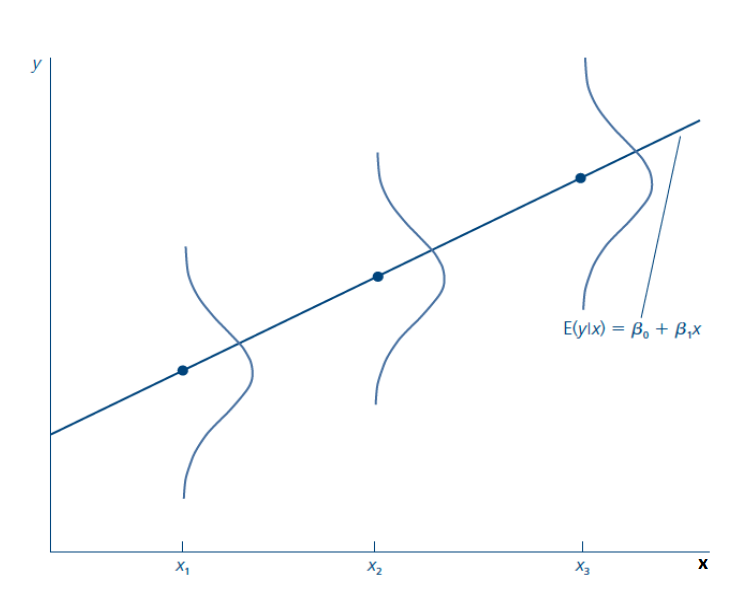
\includegraphics[width=0.7\linewidth]{../Imagenes/FRP.png}
\end{figure}
\end{frame}	

\begin{frame}
	\frametitle{Interpretaci\'on} % Título de la nueva diapositiva
\begin{equation*}
  y = \beta_0 + \beta_1x + u
\end{equation*}

\begin{equation*}
  E[y|x] = \beta_0 + \beta_1x
\end{equation*}

Noten que:

\begin{equation*}
  \beta_1 = \frac{\Delta E[y|x]}{\Delta x}
\end{equation*}

$\rightarrow$ es la pendiente de la Función de la FRP, cuando \(x\) aumenta en una unidad, el valor esperado de \(y\) cambia en \(\beta_1\) unidades.

\begin{equation*}
  \beta_0 = E[y|x = 0]
\end{equation*}

$\rightarrow$ es el intercepto de la FRP, el valor medio de \(y\) cuando \(x\) es igual a cero.

\end{frame}	

\begin{frame}
	\frametitle{Estimaci\'on} % Título de la nueva diapositiva
\begin{itemize}
  \item Objetivo: estimar los parámetros poblacionales a partir de una muestra.
  \item Sea el modelo poblacional: $y = \beta_0 + \beta_1x + u$
  \item Entonces, para cada $i = 1, \ldots, n$ de una muestra podemos escribir:
  \begin{equation*}
    y_i = \beta_0 + \beta_1x_i + u_i
  \end{equation*}
  donde $u_i$ es el término de error para la observación $i$.
\end{itemize}
\end{frame}	

\begin{frame}
	\frametitle{Mínimos Cuadrados Ordinarios}  % Título de la nueva diapositiva
%Para cada observación de la muestra se tiene la ecuación:
\[ {y}_i = \hat{\beta}_0 + \hat{\beta}_1 x_i + \hat{u}_i \quad \forall i = 1, \ldots, n \]
Definiciones:
\begin{itemize}
    \item $\hat{\beta}_0$: estimador de $\beta_0$
    \item $\hat{\beta}_1$: estimador de $\beta_1$
    \item $\hat{y}_i = \hat{\beta}_0 + \hat{\beta}_1 x_i$: valor predicho/estimado de $y_i$
    \item $\hat{u}_i = y_i - \hat{y}_i$ residuo. El residuo es el análogo muestral del error.
    \item MCO encuentra los valores de \(\hat{\beta}_0\) y \(\hat{\beta}_1\) que minimizan la suma de residuos al cuadrado:
\[ \min_{\hat{\beta}_0, \hat{\beta}_1} \sum_{i=1}^{n} \hat{u}_i^2 = \min_{\hat{\beta}_0, \hat{\beta}_1} \sum_{i=1}^{n} (y_i - \hat{\beta}_0 - \hat{\beta}_1 x_i)^2 \]
\end{itemize}
\end{frame}	




\begin{frame}
	\frametitle{Estimaci\'on de $\beta$ MCO} % Título de la nueva diapositiva
\begin{equation*}
\quad \min_{\hat{\beta}_0, \hat{\beta}_1} \sum_{i=1}^{n} \hat{u}_i^2 = \min_{\hat{\beta}_0, \hat{\beta}_1} \sum_{i=1}^{n} (y_i - \hat{\beta}_0 - \hat{\beta}_1 x_i)^2
\end{equation*}

Condiciones de primer orden:
{\small
\begin{equation*}
[\hat{\beta}_0] : \quad \sum_{i=1}^{n} (y_i - \hat{\beta}_0 - \hat{\beta}_1 x_i) = 0 \quad \Rightarrow \quad \hat{\beta}_0 = \bar{y} - \hat{\beta}_1 \bar{x} 
\end{equation*}
\begin{equation*}
[\hat{\beta}_1] : \quad \sum_{i=1}^{n} x_i(y_i - \hat{\beta}_0 - \hat{\beta}_1 x_i) = 0 \Rightarrow \hat{\beta}_1 = \frac{\sum_{i=1}^{n}(x_i - \bar{x})y_i}{\sum_{i=1}^{n}(x_i - \bar{x})^2} = \frac{\text{Cov}(x, y)}{\text{Var}(x)} 
\end{equation*}}

Noten que todas estas variables están en la data. Entonces podemos obtener estos estimadores.

\end{frame}

\begin{frame}
	\frametitle{Tarea } % Título de la nueva diapositiva
 	\begin{itemize}
  \item Muestre que:
  
  $\sum_{i}^n(x_i - \bar{x})(y_i - \bar{y}) = \sum_{i}^n(x_i - \bar{x})y_i= \sum_{i}^n(y_i - \bar{y})x_i$.
%\item Resuelvan el sistema de 2 ecuaciones y 2 incógnitas y lleguen a la misma expresión para $\beta_1$.
 	\end{itemize}
\end{frame}

\begin{frame}
	\frametitle{Regresión Muestral (FRM)} % Título de la nueva diapositiva
	\begin{enumerate}
		\item Una vez que estimamos $\hat{\beta}_0$ y $\hat{\beta}_1$, obtenemos la función de regresión muestral (FRM):
		\[ \hat{y} = \hat{\beta}_0 + \hat{\beta}_1 x \]
		
		\item La FRM que se obtiene de una muestra es la versión estimada de la función de regresión poblacional (FRP).
		
		\item En general, la FRP es desconocida y uno se basa en una muestra para estimarla.
		
		\item {\color{blue} Valor ajustado o predicho: $\hat{y}$.}
	\end{enumerate}
\end{frame}	

% \begin{frame}
% 	\frametitle{Regresión Muestral (MCO)} % Título de la nueva diapositiva
% \begin{figure}
%     \centering
%     
\includegraphics[width=0.8\linewidth]{clase2/images/regmco.png}
%     % \caption{Enter Caption}
%     \label{fig:enter-label}
% \end{figure}
% \end{frame}	

\begin{frame}
	\frametitle{Mínimos Cuadrados Ordinarios} % Título de la nueva diapositiva
\begin{figure}
    \centering
    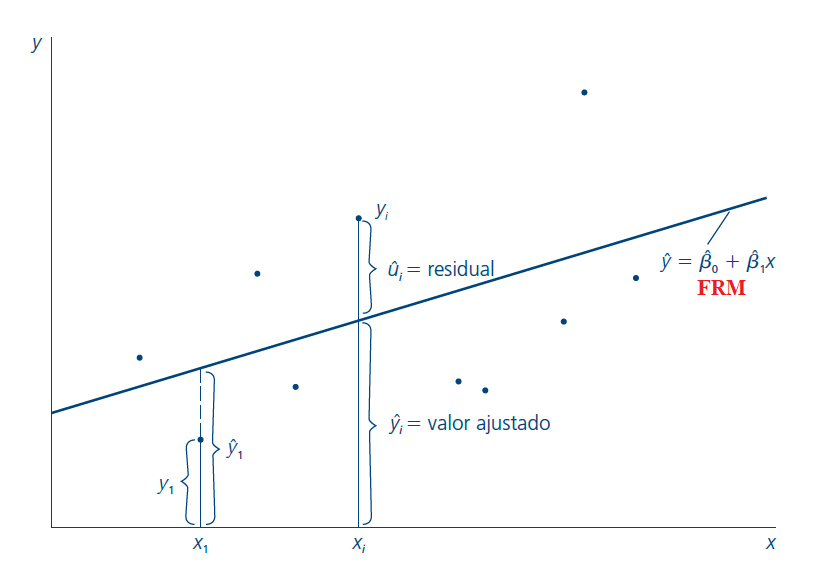
\includegraphics[width=0.9\linewidth]{images/mco.png}
    % \caption{Enter Caption}
    \label{fig:enter-label}
\end{figure}
\end{frame}	


\begin{frame}
    \frametitle{Un ejemplo: relaci\'on entre educaci\'on y sueldos}
    
    \begin{columns}
        % Columna izquierda: Texto
        \column{0.5\textwidth}
        \begin{itemize}
            \item Tomamos la relación entre años de educación y sueldos por hora en EE. UU.
            \[ salario_i = \beta_0 + \beta_1 \text{educación}_i + \epsilon_i \]
           
        \end{itemize}
        
        % Enlace debajo del texto
        \vspace{0.5cm}
        \href{https://colab.research.google.com/drive/1fGx_sLiasa-psVeudjO5IgJPPJX0lB6t?usp=sharing}{\beamergotobutton{Colab}}
        
        % Columna derecha: Solo la imagen
        \column{0.5\textwidth}
        \begin{figure}
            \centering
            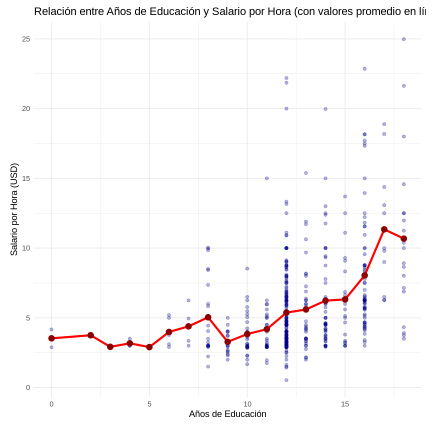
\includegraphics[width=0.9\linewidth]{images/disper1.png}
        \end{figure}
    \end{columns}

\end{frame}




\begin{frame}
	\frametitle{Un ejemplo} % Título de la nueva diapositiva
    \begin{columns}
        % Columna izquierda: Texto
        \column{0.5\textwidth}
	\begin{itemize}
		\item 	Años de educación y salarios por hora en Estados Unidos.
		\[ \widehat{salario} = 0.095 + 0.54\,educ \]
        \item La l\'inea de regresi\'on minimiza los residuos al cuadrado.
        	\end{itemize}
     \column{0.5\textwidth}    
       \begin{figure}
           \centering
           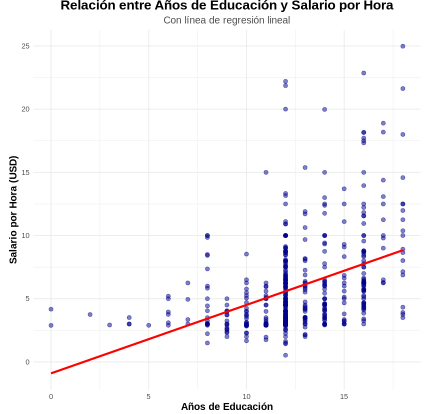
\includegraphics[width=0.75\linewidth]{images/reg.png}
       \end{figure}

   \end{columns}
\end{frame}	

\begin{frame}
	\frametitle{Propiedades aritm\'eticas de MCO} % Título de la nueva diapositiva
	\begin{enumerate}
		\item Los residuales suman cero:
		\[ \sum_{i} \hat{u}_i = 0 \quad \Rightarrow \quad \bar{\hat{u}} = 0 \]

		\item $x$ es ortogonal a los residuos:
		\[ \sum_{i} x_{i} \hat{u}_i = 0 \]

		\item El promedio muestral de la variable dependiente $y_i$ es igual al promedio muestral de la estimación $\hat{y}_i: \bar{y} = \bar{\hat{y}}$
  
		\item La línea de regresión pasa por el promedio de los datos:
		\[ \bar{y} = \hat{\beta}_0 + \hat{\beta}_1 \bar{x} \]
	\end{enumerate}
\end{frame}

\begin{frame}{Método de momentos}
\begin{eqnarray}
y=\beta_0+\beta_1x+u\\
      E(u)= 0= E(y-\beta_0-\beta_1x) \\
E(xu)=0=E[x(y-\beta_0-\beta_1x)]
\end{eqnarray}


Se eligen estimaciones de los parámetros $\beta_0$ y $\beta_1$ que resuelvan las contrapartes muestrales.

\end{frame}

\begin{frame}{Método de momentos}

\begin{eqnarray}
     \sum_{i=1}^{n} (y_i - \hat{\beta}_0 - \hat{\beta}_1 x_i) = 0  \\
 \sum_{i=1}^{n} x_i(y_i - \hat{\beta}_0 - \hat{\beta}_1 x_i) = 0 
\end{eqnarray}
    
\end{frame}



\begin{frame}
	\frametitle{Estimaci\'on de $\beta$ MCO} % Título de la nueva diapositiva
\begin{equation*}
\quad \min_{\hat{\beta}_0, \hat{\beta}_1} \sum_{i=1}^{n} \hat{u}_i^2 = \min_{\hat{\beta}_0, \hat{\beta}_1} \sum_{i=1}^{n} (y_i - \hat{\beta}_0 - \hat{\beta}_1 x_i)^2
\end{equation*}

Condiciones de primer orden:

\begin{equation*}
[\hat{\beta}_0] : \quad \sum_{i=1}^{n} (y_i - \hat{\beta}_0 - \hat{\beta}_1 x_i) = 0 
\end{equation*}
\begin{equation*}
[\hat{\beta}_1] : \quad \sum_{i=1}^{n} x_i(y_i - \hat{\beta}_0 - \hat{\beta}_1 x_i) = 0
\end{equation*}

\end{frame}


\begin{frame}
	\frametitle{Descomposición de la varianza muestral} % Título de la nueva diapositiva
	\begin{itemize}
		\item Sea SST la suma de cuadrados totales (total sum of squares):
		\[ SST = \sum_{i=1}^{n} (y_i - \bar{y})^2 \]
		
		\item Sea SSE la suma de cuadrados explicados (explained sum of squares):
		\[ SSE = \sum_{i=1}^{n} (\hat{y}_i - \bar{y})^2 \]
		
		\item Sea SSR la suma de cuadrados no explicados (residual sum of squares):
		\[ SSR = \sum_{i=1}^{n} \hat{u}_i^2 \]
	\end{itemize}
	Se puede demostrar que:
	\[ SST = SSE + SSR \]
\end{frame}	

\begin{frame}
	\frametitle{Bondad de Ajuste: $R^2$} % Título de la diapositiva
	\begin{itemize}
		\item A partir de esta relación se define:
		\[ R^2 = \frac{SSE}{SST} = 1 - \frac{SSR}{SST} \]
		
		\item Bondad de ajuste: la proporción de la varianza muestral de $y$ que es explicada por $x$.
		
		\item Como $0 \leq SSE \leq SST$, entonces $0 \leq R^2 \leq 1$.
		
		%\item El $R^2$ busca estimar el ajuste a nivel poblacional.
		
		\item Cuanto más cercano a $1$, más de la variabilidad de $y$ es explicada por el modelo.
	\end{itemize}
\end{frame}


 \begin{frame}{}

    \begin{itemize}
        \item Si la variable
 independiente se divide o se multiplica por una constante distinta de cero, c, entonces el coeficiente
de la pendiente de MCO se multiplica por c o se divide entre c, respectivamente.


\item Cambiar sólo las unidades de medición de la variable independiente no afecta el intercepto.
\item  La bondad de ajuste del modelo no
 depende de las unidades de medición de las variables.
    \end{itemize}
    
 \end{frame}



\begin{frame}{Supuesto 1 RLS}
    En el modelo poblacional, la variable dependiente, y, está relacionada con la variable independiente,
x, y con el error (o perturbación), u, de la manera siguiente:\\
$$y=\beta_0 +\beta_1x+ u$$ 

donde $\beta_0$ y $\beta_1$ representan los parámetros poblacionales, del intercepto y pendiente, respectivamente.

$u$ contiene los efectos no observables que afectan a $y$, $u$ no debe confundirse con los residuales. 

\end{frame}


\begin{frame}{Supuesto 2 RLS}
    Se cuenta con una muestra {\bf aleatoria} de tamaño n, $\lbrace(x_i,y_i): i = 1, 2, ..., n\rbrace$.


\end{frame}

\begin{frame}{Supuesto 3 RLS}
    No todos los valores muestrales de x, a saber $\lbrace x_i, i = 1,.., n\rbrace$, son iguales, es decir, no todos tienen
el mismo valor.
\end{frame}

\begin{frame}{Supuesto 4 RLS}
    Para todo valor de la variable explicativa, el valor esperado del error u es cero. 
    
$E(u|x) = 0$.
\end{frame}


\begin{frame}{Insesgamiento de los estimadores de MCO}


    Si se cumplen los supuestos 1-4 RLS, los estimadores $\hat{\beta_0}$ y $\hat{\beta_1}$ son insesgados:


$$E(\hat{\beta_0})=\beta_0$$

$$E(\hat{\beta_1})=\beta_1$$

El insesgamiento es una propiedad de las distribuciones muestrales de $\hat{\beta_0}$ y $\hat{\beta_1}$.
No dice nada acerca de las estimaciones que se obtienen a partir de una determinada
muestra. Se espera que, si la muestra es de alguna manera “representativa”, la estimación estará “cerca” del valor poblacional.
     
\end{frame}


\begin{frame}{Insesgamiento de los estimadores de MCO}
    
    \begin{itemize}
        \item Si u contiene factores que afectan a y  que están
correlacionados con x, puede obtenerse una {\color{blue} correlación espuria}.
\item Es decir, se encuentra
una relación entre  x e y que en realidad se debe a factores no observados que afectan a y  que
resultan estar correlacionados con x.
    \end{itemize}


\end{frame}


\begin{frame}{Supuesto 5 RLS}
    El error u tiene la misma varianza para cualquier valor de la variable explicativa. 
    
$$Var(u|x)=\sigma^2$$

La varianza de los
factores inobservables, u, condicionales en x, es constante. Esto se conoce como el supuesto de {\color{blue}
homocedasticidad o de varianza constante.}
\end{frame}

\begin{frame}{Varianza de los estimadores de mínimos cuadrados ordinarios}

Considerando el supuesto 5 RLS, tenemos:

$$Var(\hat{\beta_1})=\frac{\sigma^2}{\sum_{i=1}^n(x_i-\bar{x})^2} $$

$$Var(\hat{\beta_0})=\frac{\sigma^2 \sum_{i=1}^nx_i^2}{n\sum_{i=1}^n(x_i-\bar{x})^2 }$$

    
\end{frame}
\end{document}
